
% Default to the notebook output style

    


% Inherit from the specified cell style.




    
\documentclass[11pt]{article}

    
    
    \usepackage[T1]{fontenc}
    % Nicer default font (+ math font) than Computer Modern for most use cases
    \usepackage{mathpazo}

    % Basic figure setup, for now with no caption control since it's done
    % automatically by Pandoc (which extracts ![](path) syntax from Markdown).
    \usepackage{graphicx}
    % We will generate all images so they have a width \maxwidth. This means
    % that they will get their normal width if they fit onto the page, but
    % are scaled down if they would overflow the margins.
    \makeatletter
    \def\maxwidth{\ifdim\Gin@nat@width>\linewidth\linewidth
    \else\Gin@nat@width\fi}
    \makeatother
    \let\Oldincludegraphics\includegraphics
    % Set max figure width to be 80% of text width, for now hardcoded.
    \renewcommand{\includegraphics}[1]{\Oldincludegraphics[width=.8\maxwidth]{#1}}
    % Ensure that by default, figures have no caption (until we provide a
    % proper Figure object with a Caption API and a way to capture that
    % in the conversion process - todo).
    \usepackage{caption}
    \DeclareCaptionLabelFormat{nolabel}{}
    \captionsetup{labelformat=nolabel}

    \usepackage{adjustbox} % Used to constrain images to a maximum size 
    \usepackage{xcolor} % Allow colors to be defined
    \usepackage{enumerate} % Needed for markdown enumerations to work
    \usepackage{geometry} % Used to adjust the document margins
    \usepackage{amsmath} % Equations
    \usepackage{amssymb} % Equations
    \usepackage{textcomp} % defines textquotesingle
    % Hack from http://tex.stackexchange.com/a/47451/13684:
    \AtBeginDocument{%
        \def\PYZsq{\textquotesingle}% Upright quotes in Pygmentized code
    }
    \usepackage{upquote} % Upright quotes for verbatim code
    \usepackage{eurosym} % defines \euro
    \usepackage[mathletters]{ucs} % Extended unicode (utf-8) support
    \usepackage[utf8x]{inputenc} % Allow utf-8 characters in the tex document
    \usepackage{fancyvrb} % verbatim replacement that allows latex
    \usepackage{grffile} % extends the file name processing of package graphics 
                         % to support a larger range 
    % The hyperref package gives us a pdf with properly built
    % internal navigation ('pdf bookmarks' for the table of contents,
    % internal cross-reference links, web links for URLs, etc.)
    \usepackage{hyperref}
    \usepackage{longtable} % longtable support required by pandoc >1.10
    \usepackage{booktabs}  % table support for pandoc > 1.12.2
    \usepackage[inline]{enumitem} % IRkernel/repr support (it uses the enumerate* environment)
    \usepackage[normalem]{ulem} % ulem is needed to support strikethroughs (\sout)
                                % normalem makes italics be italics, not underlines
    

    
    
    % Colors for the hyperref package
    \definecolor{urlcolor}{rgb}{0,.145,.698}
    \definecolor{linkcolor}{rgb}{.71,0.21,0.01}
    \definecolor{citecolor}{rgb}{.12,.54,.11}

    % ANSI colors
    \definecolor{ansi-black}{HTML}{3E424D}
    \definecolor{ansi-black-intense}{HTML}{282C36}
    \definecolor{ansi-red}{HTML}{E75C58}
    \definecolor{ansi-red-intense}{HTML}{B22B31}
    \definecolor{ansi-green}{HTML}{00A250}
    \definecolor{ansi-green-intense}{HTML}{007427}
    \definecolor{ansi-yellow}{HTML}{DDB62B}
    \definecolor{ansi-yellow-intense}{HTML}{B27D12}
    \definecolor{ansi-blue}{HTML}{208FFB}
    \definecolor{ansi-blue-intense}{HTML}{0065CA}
    \definecolor{ansi-magenta}{HTML}{D160C4}
    \definecolor{ansi-magenta-intense}{HTML}{A03196}
    \definecolor{ansi-cyan}{HTML}{60C6C8}
    \definecolor{ansi-cyan-intense}{HTML}{258F8F}
    \definecolor{ansi-white}{HTML}{C5C1B4}
    \definecolor{ansi-white-intense}{HTML}{A1A6B2}

    % commands and environments needed by pandoc snippets
    % extracted from the output of `pandoc -s`
    \providecommand{\tightlist}{%
      \setlength{\itemsep}{0pt}\setlength{\parskip}{0pt}}
    \DefineVerbatimEnvironment{Highlighting}{Verbatim}{commandchars=\\\{\}}
    % Add ',fontsize=\small' for more characters per line
    \newenvironment{Shaded}{}{}
    \newcommand{\KeywordTok}[1]{\textcolor[rgb]{0.00,0.44,0.13}{\textbf{{#1}}}}
    \newcommand{\DataTypeTok}[1]{\textcolor[rgb]{0.56,0.13,0.00}{{#1}}}
    \newcommand{\DecValTok}[1]{\textcolor[rgb]{0.25,0.63,0.44}{{#1}}}
    \newcommand{\BaseNTok}[1]{\textcolor[rgb]{0.25,0.63,0.44}{{#1}}}
    \newcommand{\FloatTok}[1]{\textcolor[rgb]{0.25,0.63,0.44}{{#1}}}
    \newcommand{\CharTok}[1]{\textcolor[rgb]{0.25,0.44,0.63}{{#1}}}
    \newcommand{\StringTok}[1]{\textcolor[rgb]{0.25,0.44,0.63}{{#1}}}
    \newcommand{\CommentTok}[1]{\textcolor[rgb]{0.38,0.63,0.69}{\textit{{#1}}}}
    \newcommand{\OtherTok}[1]{\textcolor[rgb]{0.00,0.44,0.13}{{#1}}}
    \newcommand{\AlertTok}[1]{\textcolor[rgb]{1.00,0.00,0.00}{\textbf{{#1}}}}
    \newcommand{\FunctionTok}[1]{\textcolor[rgb]{0.02,0.16,0.49}{{#1}}}
    \newcommand{\RegionMarkerTok}[1]{{#1}}
    \newcommand{\ErrorTok}[1]{\textcolor[rgb]{1.00,0.00,0.00}{\textbf{{#1}}}}
    \newcommand{\NormalTok}[1]{{#1}}
    
    % Additional commands for more recent versions of Pandoc
    \newcommand{\ConstantTok}[1]{\textcolor[rgb]{0.53,0.00,0.00}{{#1}}}
    \newcommand{\SpecialCharTok}[1]{\textcolor[rgb]{0.25,0.44,0.63}{{#1}}}
    \newcommand{\VerbatimStringTok}[1]{\textcolor[rgb]{0.25,0.44,0.63}{{#1}}}
    \newcommand{\SpecialStringTok}[1]{\textcolor[rgb]{0.73,0.40,0.53}{{#1}}}
    \newcommand{\ImportTok}[1]{{#1}}
    \newcommand{\DocumentationTok}[1]{\textcolor[rgb]{0.73,0.13,0.13}{\textit{{#1}}}}
    \newcommand{\AnnotationTok}[1]{\textcolor[rgb]{0.38,0.63,0.69}{\textbf{\textit{{#1}}}}}
    \newcommand{\CommentVarTok}[1]{\textcolor[rgb]{0.38,0.63,0.69}{\textbf{\textit{{#1}}}}}
    \newcommand{\VariableTok}[1]{\textcolor[rgb]{0.10,0.09,0.49}{{#1}}}
    \newcommand{\ControlFlowTok}[1]{\textcolor[rgb]{0.00,0.44,0.13}{\textbf{{#1}}}}
    \newcommand{\OperatorTok}[1]{\textcolor[rgb]{0.40,0.40,0.40}{{#1}}}
    \newcommand{\BuiltInTok}[1]{{#1}}
    \newcommand{\ExtensionTok}[1]{{#1}}
    \newcommand{\PreprocessorTok}[1]{\textcolor[rgb]{0.74,0.48,0.00}{{#1}}}
    \newcommand{\AttributeTok}[1]{\textcolor[rgb]{0.49,0.56,0.16}{{#1}}}
    \newcommand{\InformationTok}[1]{\textcolor[rgb]{0.38,0.63,0.69}{\textbf{\textit{{#1}}}}}
    \newcommand{\WarningTok}[1]{\textcolor[rgb]{0.38,0.63,0.69}{\textbf{\textit{{#1}}}}}
    
    
    % Define a nice break command that doesn't care if a line doesn't already
    % exist.
    \def\br{\hspace*{\fill} \\* }
    % Math Jax compatability definitions
    \def\gt{>}
    \def\lt{<}
    % Document parameters
    \title{HW4}
    
    
    

    % Pygments definitions
    
\makeatletter
\def\PY@reset{\let\PY@it=\relax \let\PY@bf=\relax%
    \let\PY@ul=\relax \let\PY@tc=\relax%
    \let\PY@bc=\relax \let\PY@ff=\relax}
\def\PY@tok#1{\csname PY@tok@#1\endcsname}
\def\PY@toks#1+{\ifx\relax#1\empty\else%
    \PY@tok{#1}\expandafter\PY@toks\fi}
\def\PY@do#1{\PY@bc{\PY@tc{\PY@ul{%
    \PY@it{\PY@bf{\PY@ff{#1}}}}}}}
\def\PY#1#2{\PY@reset\PY@toks#1+\relax+\PY@do{#2}}

\expandafter\def\csname PY@tok@w\endcsname{\def\PY@tc##1{\textcolor[rgb]{0.73,0.73,0.73}{##1}}}
\expandafter\def\csname PY@tok@c\endcsname{\let\PY@it=\textit\def\PY@tc##1{\textcolor[rgb]{0.25,0.50,0.50}{##1}}}
\expandafter\def\csname PY@tok@cp\endcsname{\def\PY@tc##1{\textcolor[rgb]{0.74,0.48,0.00}{##1}}}
\expandafter\def\csname PY@tok@k\endcsname{\let\PY@bf=\textbf\def\PY@tc##1{\textcolor[rgb]{0.00,0.50,0.00}{##1}}}
\expandafter\def\csname PY@tok@kp\endcsname{\def\PY@tc##1{\textcolor[rgb]{0.00,0.50,0.00}{##1}}}
\expandafter\def\csname PY@tok@kt\endcsname{\def\PY@tc##1{\textcolor[rgb]{0.69,0.00,0.25}{##1}}}
\expandafter\def\csname PY@tok@o\endcsname{\def\PY@tc##1{\textcolor[rgb]{0.40,0.40,0.40}{##1}}}
\expandafter\def\csname PY@tok@ow\endcsname{\let\PY@bf=\textbf\def\PY@tc##1{\textcolor[rgb]{0.67,0.13,1.00}{##1}}}
\expandafter\def\csname PY@tok@nb\endcsname{\def\PY@tc##1{\textcolor[rgb]{0.00,0.50,0.00}{##1}}}
\expandafter\def\csname PY@tok@nf\endcsname{\def\PY@tc##1{\textcolor[rgb]{0.00,0.00,1.00}{##1}}}
\expandafter\def\csname PY@tok@nc\endcsname{\let\PY@bf=\textbf\def\PY@tc##1{\textcolor[rgb]{0.00,0.00,1.00}{##1}}}
\expandafter\def\csname PY@tok@nn\endcsname{\let\PY@bf=\textbf\def\PY@tc##1{\textcolor[rgb]{0.00,0.00,1.00}{##1}}}
\expandafter\def\csname PY@tok@ne\endcsname{\let\PY@bf=\textbf\def\PY@tc##1{\textcolor[rgb]{0.82,0.25,0.23}{##1}}}
\expandafter\def\csname PY@tok@nv\endcsname{\def\PY@tc##1{\textcolor[rgb]{0.10,0.09,0.49}{##1}}}
\expandafter\def\csname PY@tok@no\endcsname{\def\PY@tc##1{\textcolor[rgb]{0.53,0.00,0.00}{##1}}}
\expandafter\def\csname PY@tok@nl\endcsname{\def\PY@tc##1{\textcolor[rgb]{0.63,0.63,0.00}{##1}}}
\expandafter\def\csname PY@tok@ni\endcsname{\let\PY@bf=\textbf\def\PY@tc##1{\textcolor[rgb]{0.60,0.60,0.60}{##1}}}
\expandafter\def\csname PY@tok@na\endcsname{\def\PY@tc##1{\textcolor[rgb]{0.49,0.56,0.16}{##1}}}
\expandafter\def\csname PY@tok@nt\endcsname{\let\PY@bf=\textbf\def\PY@tc##1{\textcolor[rgb]{0.00,0.50,0.00}{##1}}}
\expandafter\def\csname PY@tok@nd\endcsname{\def\PY@tc##1{\textcolor[rgb]{0.67,0.13,1.00}{##1}}}
\expandafter\def\csname PY@tok@s\endcsname{\def\PY@tc##1{\textcolor[rgb]{0.73,0.13,0.13}{##1}}}
\expandafter\def\csname PY@tok@sd\endcsname{\let\PY@it=\textit\def\PY@tc##1{\textcolor[rgb]{0.73,0.13,0.13}{##1}}}
\expandafter\def\csname PY@tok@si\endcsname{\let\PY@bf=\textbf\def\PY@tc##1{\textcolor[rgb]{0.73,0.40,0.53}{##1}}}
\expandafter\def\csname PY@tok@se\endcsname{\let\PY@bf=\textbf\def\PY@tc##1{\textcolor[rgb]{0.73,0.40,0.13}{##1}}}
\expandafter\def\csname PY@tok@sr\endcsname{\def\PY@tc##1{\textcolor[rgb]{0.73,0.40,0.53}{##1}}}
\expandafter\def\csname PY@tok@ss\endcsname{\def\PY@tc##1{\textcolor[rgb]{0.10,0.09,0.49}{##1}}}
\expandafter\def\csname PY@tok@sx\endcsname{\def\PY@tc##1{\textcolor[rgb]{0.00,0.50,0.00}{##1}}}
\expandafter\def\csname PY@tok@m\endcsname{\def\PY@tc##1{\textcolor[rgb]{0.40,0.40,0.40}{##1}}}
\expandafter\def\csname PY@tok@gh\endcsname{\let\PY@bf=\textbf\def\PY@tc##1{\textcolor[rgb]{0.00,0.00,0.50}{##1}}}
\expandafter\def\csname PY@tok@gu\endcsname{\let\PY@bf=\textbf\def\PY@tc##1{\textcolor[rgb]{0.50,0.00,0.50}{##1}}}
\expandafter\def\csname PY@tok@gd\endcsname{\def\PY@tc##1{\textcolor[rgb]{0.63,0.00,0.00}{##1}}}
\expandafter\def\csname PY@tok@gi\endcsname{\def\PY@tc##1{\textcolor[rgb]{0.00,0.63,0.00}{##1}}}
\expandafter\def\csname PY@tok@gr\endcsname{\def\PY@tc##1{\textcolor[rgb]{1.00,0.00,0.00}{##1}}}
\expandafter\def\csname PY@tok@ge\endcsname{\let\PY@it=\textit}
\expandafter\def\csname PY@tok@gs\endcsname{\let\PY@bf=\textbf}
\expandafter\def\csname PY@tok@gp\endcsname{\let\PY@bf=\textbf\def\PY@tc##1{\textcolor[rgb]{0.00,0.00,0.50}{##1}}}
\expandafter\def\csname PY@tok@go\endcsname{\def\PY@tc##1{\textcolor[rgb]{0.53,0.53,0.53}{##1}}}
\expandafter\def\csname PY@tok@gt\endcsname{\def\PY@tc##1{\textcolor[rgb]{0.00,0.27,0.87}{##1}}}
\expandafter\def\csname PY@tok@err\endcsname{\def\PY@bc##1{\setlength{\fboxsep}{0pt}\fcolorbox[rgb]{1.00,0.00,0.00}{1,1,1}{\strut ##1}}}
\expandafter\def\csname PY@tok@kc\endcsname{\let\PY@bf=\textbf\def\PY@tc##1{\textcolor[rgb]{0.00,0.50,0.00}{##1}}}
\expandafter\def\csname PY@tok@kd\endcsname{\let\PY@bf=\textbf\def\PY@tc##1{\textcolor[rgb]{0.00,0.50,0.00}{##1}}}
\expandafter\def\csname PY@tok@kn\endcsname{\let\PY@bf=\textbf\def\PY@tc##1{\textcolor[rgb]{0.00,0.50,0.00}{##1}}}
\expandafter\def\csname PY@tok@kr\endcsname{\let\PY@bf=\textbf\def\PY@tc##1{\textcolor[rgb]{0.00,0.50,0.00}{##1}}}
\expandafter\def\csname PY@tok@bp\endcsname{\def\PY@tc##1{\textcolor[rgb]{0.00,0.50,0.00}{##1}}}
\expandafter\def\csname PY@tok@fm\endcsname{\def\PY@tc##1{\textcolor[rgb]{0.00,0.00,1.00}{##1}}}
\expandafter\def\csname PY@tok@vc\endcsname{\def\PY@tc##1{\textcolor[rgb]{0.10,0.09,0.49}{##1}}}
\expandafter\def\csname PY@tok@vg\endcsname{\def\PY@tc##1{\textcolor[rgb]{0.10,0.09,0.49}{##1}}}
\expandafter\def\csname PY@tok@vi\endcsname{\def\PY@tc##1{\textcolor[rgb]{0.10,0.09,0.49}{##1}}}
\expandafter\def\csname PY@tok@vm\endcsname{\def\PY@tc##1{\textcolor[rgb]{0.10,0.09,0.49}{##1}}}
\expandafter\def\csname PY@tok@sa\endcsname{\def\PY@tc##1{\textcolor[rgb]{0.73,0.13,0.13}{##1}}}
\expandafter\def\csname PY@tok@sb\endcsname{\def\PY@tc##1{\textcolor[rgb]{0.73,0.13,0.13}{##1}}}
\expandafter\def\csname PY@tok@sc\endcsname{\def\PY@tc##1{\textcolor[rgb]{0.73,0.13,0.13}{##1}}}
\expandafter\def\csname PY@tok@dl\endcsname{\def\PY@tc##1{\textcolor[rgb]{0.73,0.13,0.13}{##1}}}
\expandafter\def\csname PY@tok@s2\endcsname{\def\PY@tc##1{\textcolor[rgb]{0.73,0.13,0.13}{##1}}}
\expandafter\def\csname PY@tok@sh\endcsname{\def\PY@tc##1{\textcolor[rgb]{0.73,0.13,0.13}{##1}}}
\expandafter\def\csname PY@tok@s1\endcsname{\def\PY@tc##1{\textcolor[rgb]{0.73,0.13,0.13}{##1}}}
\expandafter\def\csname PY@tok@mb\endcsname{\def\PY@tc##1{\textcolor[rgb]{0.40,0.40,0.40}{##1}}}
\expandafter\def\csname PY@tok@mf\endcsname{\def\PY@tc##1{\textcolor[rgb]{0.40,0.40,0.40}{##1}}}
\expandafter\def\csname PY@tok@mh\endcsname{\def\PY@tc##1{\textcolor[rgb]{0.40,0.40,0.40}{##1}}}
\expandafter\def\csname PY@tok@mi\endcsname{\def\PY@tc##1{\textcolor[rgb]{0.40,0.40,0.40}{##1}}}
\expandafter\def\csname PY@tok@il\endcsname{\def\PY@tc##1{\textcolor[rgb]{0.40,0.40,0.40}{##1}}}
\expandafter\def\csname PY@tok@mo\endcsname{\def\PY@tc##1{\textcolor[rgb]{0.40,0.40,0.40}{##1}}}
\expandafter\def\csname PY@tok@ch\endcsname{\let\PY@it=\textit\def\PY@tc##1{\textcolor[rgb]{0.25,0.50,0.50}{##1}}}
\expandafter\def\csname PY@tok@cm\endcsname{\let\PY@it=\textit\def\PY@tc##1{\textcolor[rgb]{0.25,0.50,0.50}{##1}}}
\expandafter\def\csname PY@tok@cpf\endcsname{\let\PY@it=\textit\def\PY@tc##1{\textcolor[rgb]{0.25,0.50,0.50}{##1}}}
\expandafter\def\csname PY@tok@c1\endcsname{\let\PY@it=\textit\def\PY@tc##1{\textcolor[rgb]{0.25,0.50,0.50}{##1}}}
\expandafter\def\csname PY@tok@cs\endcsname{\let\PY@it=\textit\def\PY@tc##1{\textcolor[rgb]{0.25,0.50,0.50}{##1}}}

\def\PYZbs{\char`\\}
\def\PYZus{\char`\_}
\def\PYZob{\char`\{}
\def\PYZcb{\char`\}}
\def\PYZca{\char`\^}
\def\PYZam{\char`\&}
\def\PYZlt{\char`\<}
\def\PYZgt{\char`\>}
\def\PYZsh{\char`\#}
\def\PYZpc{\char`\%}
\def\PYZdl{\char`\$}
\def\PYZhy{\char`\-}
\def\PYZsq{\char`\'}
\def\PYZdq{\char`\"}
\def\PYZti{\char`\~}
% for compatibility with earlier versions
\def\PYZat{@}
\def\PYZlb{[}
\def\PYZrb{]}
\makeatother


    % Exact colors from NB
    \definecolor{incolor}{rgb}{0.0, 0.0, 0.5}
    \definecolor{outcolor}{rgb}{0.545, 0.0, 0.0}



    
    % Prevent overflowing lines due to hard-to-break entities
    \sloppy 
    % Setup hyperref package
    \hypersetup{
      breaklinks=true,  % so long urls are correctly broken across lines
      colorlinks=true,
      urlcolor=urlcolor,
      linkcolor=linkcolor,
      citecolor=citecolor,
      }
    % Slightly bigger margins than the latex defaults
    
    \geometry{verbose,tmargin=1in,bmargin=1in,lmargin=1in,rmargin=1in}
    
    

    \begin{document}
    
    
    \maketitle
    
    

    
    \subsubsection{Homework 4}\label{homework-4}

    \paragraph{Erin Witmer}\label{erin-witmer}

CSC 440

    \paragraph{{[}8.3{]} Given a decision tree, you have the option of (a)
converting the decision tree to rules and then pruning the resulting
rules, or (b) pruning the decision tree and then converting the pruned
tree into rules. What advantage does (a) have over
(b)?}\label{given-a-decision-tree-you-have-the-option-of-a-converting-the-decision-tree-to-rules-and-then-pruning-the-resulting-rules-or-b-pruning-the-decision-tree-and-then-converting-the-pruned-tree-into-rules.-what-advantage-does-a-have-over-b}

    A decision tree can be converted to IF-THEN rules by tracing the path
from the root node to each leaf in the tree. If the tree is pruned
before the rules are created, as is suggested in case (b), then any path
dependent on the trimmed node will also be trimmed. First creating the
rules, and then trimming them as proposed in (a) allows for more
precision when trimming. Leaves dependent on a specific preceding node
may be trimmed, while other leaves dependent on that same preceding node
may be kept. However, it is important to note the higher computational
complexity associated with building a full tree, converting to rules and
then trimming. Regardless, method (a) generally generates a more precise
and accurate set of rules and is worth the computational cost.

    \begin{figure}
\centering
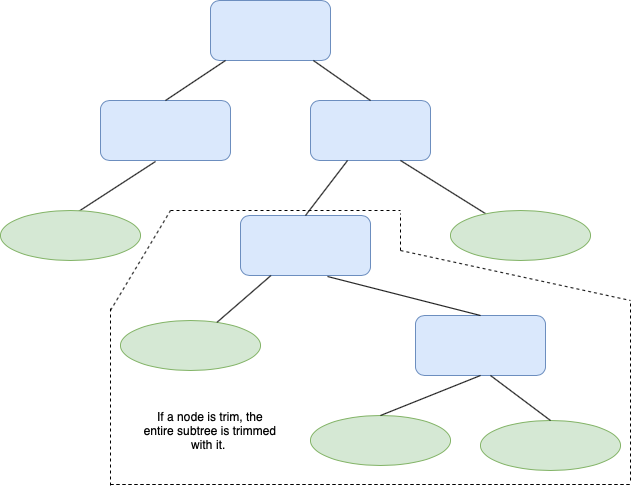
\includegraphics{tree.png}
\caption{}
\end{figure}

    \paragraph{{[}8.5{]} Given a 5-GB data set with 50 attributes (each
containing 100 distinct values) and 512 MB of main memory in your
laptop, outline an efficient method that constructs decision trees in
such large data sets. Justify your answer by rough calculation of your
main memory
usage.}\label{given-a-5-gb-data-set-with-50-attributes-each-containing-100-distinct-values-and-512-mb-of-main-memory-in-your-laptop-outline-an-efficient-method-that-constructs-decision-trees-in-such-large-data-sets.-justify-your-answer-by-rough-calculation-of-your-main-memory-usage.}

    The use of the RainForest algorithm would be most effective in this
case. RainForest adapts to the amount of main memory available and
applies to any decision tree induction algorithm. The first step is to
construct an AVC-set for each attribute. If the total data set is 5MB,
on average each attribute would be 100MB. The process would be to
extract one attribute, calculate the AVC, and store that set in main
memory. On average, if you assume you are storing the value/class count
as an integer (4 bytes), there are 100 values per attribute, and assume
there are 2 class outcomes, an individual AVC set would require
approximate (100 x 2 x 4 bytes) = 800 bytes. So the data holding the
aggregate information from which the decision tree can be constructed is
only 40 KB. Since this is the aggregate data, every level of the tree
will be some derivative of this data. Utilizing the basic algorithm for
inducing a decision tree, you could loop through many times without
running out of memory. If the tree got very deep and space was an issue,
tree prunning could take place while the tree is being generated and
only summary information could be retained at each level.

    \paragraph{{[}8.7{]} The following table consists of training data from
an employee database. The data have been
generalized....}\label{the-following-table-consists-of-training-data-from-an-employee-database.-the-data-have-been-generalized....}

    \begin{Verbatim}[commandchars=\\\{\}]
{\color{incolor}In [{\color{incolor}1}]:} \PY{n}{data} \PY{o}{=} \PY{p}{\PYZob{}}\PY{l+s+s1}{\PYZsq{}}\PY{l+s+s1}{t0}\PY{l+s+s1}{\PYZsq{}}\PY{p}{:} \PY{p}{[}\PY{l+s+s1}{\PYZsq{}}\PY{l+s+s1}{sales}\PY{l+s+s1}{\PYZsq{}}\PY{p}{,} \PY{l+s+s1}{\PYZsq{}}\PY{l+s+s1}{senior}\PY{l+s+s1}{\PYZsq{}}\PY{p}{,} \PY{l+s+s1}{\PYZsq{}}\PY{l+s+s1}{31…35}\PY{l+s+s1}{\PYZsq{}}\PY{p}{,} \PY{l+s+s1}{\PYZsq{}}\PY{l+s+s1}{46K…50K}\PY{l+s+s1}{\PYZsq{}}\PY{p}{,} \PY{l+m+mi}{30}\PY{p}{]}\PY{p}{,}
                \PY{l+s+s1}{\PYZsq{}}\PY{l+s+s1}{t1}\PY{l+s+s1}{\PYZsq{}}\PY{p}{:} \PY{p}{[}\PY{l+s+s1}{\PYZsq{}}\PY{l+s+s1}{sales}\PY{l+s+s1}{\PYZsq{}}\PY{p}{,} \PY{l+s+s1}{\PYZsq{}}\PY{l+s+s1}{junior}\PY{l+s+s1}{\PYZsq{}}\PY{p}{,} \PY{l+s+s1}{\PYZsq{}}\PY{l+s+s1}{26…30}\PY{l+s+s1}{\PYZsq{}}\PY{p}{,} \PY{l+s+s1}{\PYZsq{}}\PY{l+s+s1}{26K…30K}\PY{l+s+s1}{\PYZsq{}}\PY{p}{,} \PY{l+m+mi}{40}\PY{p}{]}\PY{p}{,}
                \PY{l+s+s1}{\PYZsq{}}\PY{l+s+s1}{t2}\PY{l+s+s1}{\PYZsq{}}\PY{p}{:} \PY{p}{[}\PY{l+s+s1}{\PYZsq{}}\PY{l+s+s1}{sales}\PY{l+s+s1}{\PYZsq{}}\PY{p}{,} \PY{l+s+s1}{\PYZsq{}}\PY{l+s+s1}{junior}\PY{l+s+s1}{\PYZsq{}}\PY{p}{,} \PY{l+s+s1}{\PYZsq{}}\PY{l+s+s1}{31…35}\PY{l+s+s1}{\PYZsq{}}\PY{p}{,} \PY{l+s+s1}{\PYZsq{}}\PY{l+s+s1}{31K…35K}\PY{l+s+s1}{\PYZsq{}}\PY{p}{,} \PY{l+m+mi}{40}\PY{p}{]}\PY{p}{,}
                \PY{l+s+s1}{\PYZsq{}}\PY{l+s+s1}{t3}\PY{l+s+s1}{\PYZsq{}}\PY{p}{:} \PY{p}{[}\PY{l+s+s1}{\PYZsq{}}\PY{l+s+s1}{systems}\PY{l+s+s1}{\PYZsq{}}\PY{p}{,} \PY{l+s+s1}{\PYZsq{}}\PY{l+s+s1}{junior}\PY{l+s+s1}{\PYZsq{}}\PY{p}{,} \PY{l+s+s1}{\PYZsq{}}\PY{l+s+s1}{21…25}\PY{l+s+s1}{\PYZsq{}}\PY{p}{,} \PY{l+s+s1}{\PYZsq{}}\PY{l+s+s1}{46K…50K}\PY{l+s+s1}{\PYZsq{}}\PY{p}{,} \PY{l+m+mi}{20}\PY{p}{]}\PY{p}{,}
                \PY{l+s+s1}{\PYZsq{}}\PY{l+s+s1}{t4}\PY{l+s+s1}{\PYZsq{}}\PY{p}{:} \PY{p}{[}\PY{l+s+s1}{\PYZsq{}}\PY{l+s+s1}{systems}\PY{l+s+s1}{\PYZsq{}}\PY{p}{,} \PY{l+s+s1}{\PYZsq{}}\PY{l+s+s1}{senior}\PY{l+s+s1}{\PYZsq{}}\PY{p}{,} \PY{l+s+s1}{\PYZsq{}}\PY{l+s+s1}{31…35}\PY{l+s+s1}{\PYZsq{}}\PY{p}{,} \PY{l+s+s1}{\PYZsq{}}\PY{l+s+s1}{66K…70K}\PY{l+s+s1}{\PYZsq{}}\PY{p}{,} \PY{l+m+mi}{5}\PY{p}{]}\PY{p}{,}
                \PY{l+s+s1}{\PYZsq{}}\PY{l+s+s1}{t5}\PY{l+s+s1}{\PYZsq{}}\PY{p}{:} \PY{p}{[}\PY{l+s+s1}{\PYZsq{}}\PY{l+s+s1}{systems}\PY{l+s+s1}{\PYZsq{}}\PY{p}{,} \PY{l+s+s1}{\PYZsq{}}\PY{l+s+s1}{junior}\PY{l+s+s1}{\PYZsq{}}\PY{p}{,} \PY{l+s+s1}{\PYZsq{}}\PY{l+s+s1}{26…30}\PY{l+s+s1}{\PYZsq{}}\PY{p}{,} \PY{l+s+s1}{\PYZsq{}}\PY{l+s+s1}{46K…50K}\PY{l+s+s1}{\PYZsq{}}\PY{p}{,} \PY{l+m+mi}{3}\PY{p}{]}\PY{p}{,}
                \PY{l+s+s1}{\PYZsq{}}\PY{l+s+s1}{t6}\PY{l+s+s1}{\PYZsq{}}\PY{p}{:} \PY{p}{[}\PY{l+s+s1}{\PYZsq{}}\PY{l+s+s1}{systems}\PY{l+s+s1}{\PYZsq{}}\PY{p}{,} \PY{l+s+s1}{\PYZsq{}}\PY{l+s+s1}{senior}\PY{l+s+s1}{\PYZsq{}}\PY{p}{,} \PY{l+s+s1}{\PYZsq{}}\PY{l+s+s1}{41…45}\PY{l+s+s1}{\PYZsq{}}\PY{p}{,} \PY{l+s+s1}{\PYZsq{}}\PY{l+s+s1}{66K…70K}\PY{l+s+s1}{\PYZsq{}}\PY{p}{,} \PY{l+m+mi}{3}\PY{p}{]}\PY{p}{,}
                \PY{l+s+s1}{\PYZsq{}}\PY{l+s+s1}{t7}\PY{l+s+s1}{\PYZsq{}}\PY{p}{:} \PY{p}{[}\PY{l+s+s1}{\PYZsq{}}\PY{l+s+s1}{marketing}\PY{l+s+s1}{\PYZsq{}}\PY{p}{,} \PY{l+s+s1}{\PYZsq{}}\PY{l+s+s1}{senior}\PY{l+s+s1}{\PYZsq{}}\PY{p}{,} \PY{l+s+s1}{\PYZsq{}}\PY{l+s+s1}{36…40}\PY{l+s+s1}{\PYZsq{}}\PY{p}{,} \PY{l+s+s1}{\PYZsq{}}\PY{l+s+s1}{46K…50K}\PY{l+s+s1}{\PYZsq{}}\PY{p}{,} \PY{l+m+mi}{10}\PY{p}{]}\PY{p}{,}
                \PY{l+s+s1}{\PYZsq{}}\PY{l+s+s1}{t8}\PY{l+s+s1}{\PYZsq{}}\PY{p}{:} \PY{p}{[}\PY{l+s+s1}{\PYZsq{}}\PY{l+s+s1}{marketing}\PY{l+s+s1}{\PYZsq{}}\PY{p}{,} \PY{l+s+s1}{\PYZsq{}}\PY{l+s+s1}{junior}\PY{l+s+s1}{\PYZsq{}}\PY{p}{,} \PY{l+s+s1}{\PYZsq{}}\PY{l+s+s1}{31…35}\PY{l+s+s1}{\PYZsq{}}\PY{p}{,} \PY{l+s+s1}{\PYZsq{}}\PY{l+s+s1}{41K…45K}\PY{l+s+s1}{\PYZsq{}}\PY{p}{,} \PY{l+m+mi}{4}\PY{p}{]}\PY{p}{,}
                \PY{l+s+s1}{\PYZsq{}}\PY{l+s+s1}{t9}\PY{l+s+s1}{\PYZsq{}}\PY{p}{:} \PY{p}{[}\PY{l+s+s1}{\PYZsq{}}\PY{l+s+s1}{secretary}\PY{l+s+s1}{\PYZsq{}}\PY{p}{,} \PY{l+s+s1}{\PYZsq{}}\PY{l+s+s1}{senior}\PY{l+s+s1}{\PYZsq{}}\PY{p}{,} \PY{l+s+s1}{\PYZsq{}}\PY{l+s+s1}{46…50}\PY{l+s+s1}{\PYZsq{}}\PY{p}{,} \PY{l+s+s1}{\PYZsq{}}\PY{l+s+s1}{36K…40K}\PY{l+s+s1}{\PYZsq{}}\PY{p}{,} \PY{l+m+mi}{4}\PY{p}{]}\PY{p}{,}
                \PY{l+s+s1}{\PYZsq{}}\PY{l+s+s1}{t10}\PY{l+s+s1}{\PYZsq{}}\PY{p}{:} \PY{p}{[}\PY{l+s+s1}{\PYZsq{}}\PY{l+s+s1}{secretary}\PY{l+s+s1}{\PYZsq{}}\PY{p}{,} \PY{l+s+s1}{\PYZsq{}}\PY{l+s+s1}{junior}\PY{l+s+s1}{\PYZsq{}}\PY{p}{,} \PY{l+s+s1}{\PYZsq{}}\PY{l+s+s1}{26…30}\PY{l+s+s1}{\PYZsq{}}\PY{p}{,} \PY{l+s+s1}{\PYZsq{}}\PY{l+s+s1}{26K…30K}\PY{l+s+s1}{\PYZsq{}}\PY{p}{,} \PY{l+m+mi}{6}\PY{p}{]}\PY{p}{\PYZcb{}}
\end{Verbatim}


    \paragraph{(a.) How would you modify the basic decision tree algorithm
to take into consideration the count of each generalized data
tuple?}\label{a.-how-would-you-modify-the-basic-decision-tree-algorithm-to-take-into-consideration-the-count-of-each-generalized-data-tuple}

    The relative weights of each of the tuples in the entropy calculation
needs to be adjusted to reflect the proportion of the count to total
employees (sum of count).

    \paragraph{(b.) Use your algorithm to construct a decision tree from the
given
data.}\label{b.-use-your-algorithm-to-construct-a-decision-tree-from-the-given-data.}

    \begin{Verbatim}[commandchars=\\\{\}]
{\color{incolor}In [{\color{incolor}2}]:} \PY{k+kn}{import} \PY{n+nn}{pandas} \PY{k}{as} \PY{n+nn}{pd}
        \PY{k+kn}{import} \PY{n+nn}{math}
        \PY{k+kn}{from} \PY{n+nn}{functools} \PY{k}{import} \PY{n}{reduce}
        
        \PY{k}{def} \PY{n+nf}{entropy}\PY{p}{(}\PY{n}{a}\PY{p}{,}\PY{n}{b}\PY{p}{)}\PY{p}{:}
            \PY{n+nb}{sum} \PY{o}{=} \PY{n}{a}\PY{o}{+}\PY{n}{b}
            \PY{n}{total} \PY{o}{=} \PY{o}{\PYZhy{}}\PY{p}{(}\PY{n}{a}\PY{o}{/}\PY{n+nb}{sum}\PY{p}{)}\PY{o}{*}\PY{n}{math}\PY{o}{.}\PY{n}{log2}\PY{p}{(}\PY{p}{(}\PY{n}{a}\PY{o}{/}\PY{n+nb}{sum}\PY{p}{)}\PY{p}{)}\PY{o}{\PYZhy{}}\PY{p}{(}\PY{n}{b}\PY{o}{/}\PY{n+nb}{sum}\PY{p}{)}\PY{o}{*}\PY{n}{math}\PY{o}{.}\PY{n}{log2}\PY{p}{(}\PY{p}{(}\PY{n}{b}\PY{o}{/}\PY{n+nb}{sum}\PY{p}{)}\PY{p}{)}
            \PY{k}{return} \PY{n}{total}
        
        \PY{n}{df} \PY{o}{=} \PY{n}{pd}\PY{o}{.}\PY{n}{DataFrame}\PY{o}{.}\PY{n}{from\PYZus{}dict}\PY{p}{(}\PY{n}{data}\PY{p}{,} \PY{n}{orient}\PY{o}{=}\PY{l+s+s1}{\PYZsq{}}\PY{l+s+s1}{index}\PY{l+s+s1}{\PYZsq{}}\PY{p}{,} \PY{n}{columns}\PY{o}{=}\PY{p}{[}\PY{l+s+s1}{\PYZsq{}}\PY{l+s+s1}{dept}\PY{l+s+s1}{\PYZsq{}}\PY{p}{,} \PY{l+s+s1}{\PYZsq{}}\PY{l+s+s1}{class}\PY{l+s+s1}{\PYZsq{}}\PY{p}{,} \PY{l+s+s1}{\PYZsq{}}\PY{l+s+s1}{age}\PY{l+s+s1}{\PYZsq{}}\PY{p}{,} \PY{l+s+s1}{\PYZsq{}}\PY{l+s+s1}{salary}\PY{l+s+s1}{\PYZsq{}}\PY{p}{,} \PY{l+s+s1}{\PYZsq{}}\PY{l+s+s1}{count}\PY{l+s+s1}{\PYZsq{}}\PY{p}{]}\PY{p}{)}
        \PY{n}{class\PYZus{}count} \PY{o}{=} \PY{n}{df}\PY{o}{.}\PY{n}{groupby}\PY{p}{(}\PY{l+s+s1}{\PYZsq{}}\PY{l+s+s1}{class}\PY{l+s+s1}{\PYZsq{}}\PY{p}{)}\PY{o}{.}\PY{n}{sum}\PY{p}{(}\PY{p}{)}
        \PY{n+nb}{print}\PY{p}{(}\PY{n}{class\PYZus{}count}\PY{p}{)}
        \PY{n}{head} \PY{o}{=} \PY{n}{entropy}\PY{p}{(}\PY{l+m+mi}{113}\PY{p}{,}\PY{l+m+mi}{52}\PY{p}{)}
\end{Verbatim}


    \begin{Verbatim}[commandchars=\\\{\}]
        count
class        
junior    113
senior     52

    \end{Verbatim}

    \begin{Verbatim}[commandchars=\\\{\}]
{\color{incolor}In [{\color{incolor}3}]:} \PY{c+c1}{\PYZsh{} department}
        \PY{n}{dept\PYZus{}count} \PY{o}{=} \PY{n}{df}\PY{o}{.}\PY{n}{groupby}\PY{p}{(}\PY{p}{[}\PY{l+s+s1}{\PYZsq{}}\PY{l+s+s1}{dept}\PY{l+s+s1}{\PYZsq{}}\PY{p}{]}\PY{p}{)}\PY{o}{.}\PY{n}{sum}\PY{p}{(}\PY{p}{)}
        \PY{n+nb}{print}\PY{p}{(}\PY{n}{dept\PYZus{}count}\PY{p}{)}
\end{Verbatim}


    \begin{Verbatim}[commandchars=\\\{\}]
           count
dept            
marketing     14
sales        110
secretary     10
systems       31

    \end{Verbatim}

    \begin{Verbatim}[commandchars=\\\{\}]
{\color{incolor}In [{\color{incolor}4}]:} \PY{n}{sales} \PY{o}{=} \PY{l+m+mi}{110}\PY{o}{/}\PY{l+m+mi}{165} 
        \PY{n}{systems} \PY{o}{=} \PY{l+m+mi}{31}\PY{o}{/}\PY{l+m+mi}{165}
        \PY{n}{marketing} \PY{o}{=} \PY{l+m+mi}{14}\PY{o}{/}\PY{l+m+mi}{165}
        \PY{n}{secretary} \PY{o}{=} \PY{l+m+mi}{10}\PY{o}{/}\PY{l+m+mi}{165}
        
        \PY{n}{dept\PYZus{}outcome} \PY{o}{=} \PY{n}{df}\PY{o}{.}\PY{n}{groupby}\PY{p}{(}\PY{p}{[}\PY{l+s+s1}{\PYZsq{}}\PY{l+s+s1}{dept}\PY{l+s+s1}{\PYZsq{}}\PY{p}{,}\PY{l+s+s1}{\PYZsq{}}\PY{l+s+s1}{class}\PY{l+s+s1}{\PYZsq{}}\PY{p}{]}\PY{p}{)}\PY{o}{.}\PY{n}{sum}\PY{p}{(}\PY{p}{)}
        \PY{n+nb}{print}\PY{p}{(}\PY{n}{dept\PYZus{}outcome}\PY{p}{)}
\end{Verbatim}


    \begin{Verbatim}[commandchars=\\\{\}]
                  count
dept      class        
marketing junior      4
          senior     10
sales     junior     80
          senior     30
secretary junior      6
          senior      4
systems   junior     23
          senior      8

    \end{Verbatim}

    \begin{Verbatim}[commandchars=\\\{\}]
{\color{incolor}In [{\color{incolor}5}]:} \PY{n}{dept\PYZus{}gain} \PY{o}{=} \PY{n}{head} \PY{o}{\PYZhy{}} \PY{p}{(}\PY{n}{sales}\PY{o}{*}\PY{n}{entropy}\PY{p}{(}\PY{l+m+mi}{80}\PY{p}{,}\PY{l+m+mi}{30}\PY{p}{)}
                            \PY{o}{+}\PY{n}{systems}\PY{o}{*}\PY{n}{entropy}\PY{p}{(}\PY{l+m+mi}{23}\PY{p}{,}\PY{l+m+mi}{8}\PY{p}{)}
                            \PY{o}{+}\PY{n}{marketing}\PY{o}{*}\PY{n}{entropy}\PY{p}{(}\PY{l+m+mi}{4}\PY{p}{,}\PY{l+m+mi}{10}\PY{p}{)}
                            \PY{o}{+}\PY{n}{secretary}\PY{o}{*}\PY{n}{entropy}\PY{p}{(}\PY{l+m+mi}{6}\PY{p}{,}\PY{l+m+mi}{4}\PY{p}{)}\PY{p}{)}
        \PY{n+nb}{print}\PY{p}{(}\PY{n}{dept\PYZus{}gain}\PY{p}{)}
\end{Verbatim}


    \begin{Verbatim}[commandchars=\\\{\}]
0.048606785991983426

    \end{Verbatim}

    \begin{Verbatim}[commandchars=\\\{\}]
{\color{incolor}In [{\color{incolor}6}]:} \PY{c+c1}{\PYZsh{} age}
        \PY{n}{age\PYZus{}count} \PY{o}{=} \PY{n}{df}\PY{o}{.}\PY{n}{groupby}\PY{p}{(}\PY{p}{[}\PY{l+s+s1}{\PYZsq{}}\PY{l+s+s1}{age}\PY{l+s+s1}{\PYZsq{}}\PY{p}{]}\PY{p}{)}\PY{o}{.}\PY{n}{sum}\PY{p}{(}\PY{p}{)}
        \PY{n+nb}{print}\PY{p}{(}\PY{n}{age\PYZus{}count}\PY{p}{)}
\end{Verbatim}


    \begin{Verbatim}[commandchars=\\\{\}]
       count
age         
21…25     20
26…30     49
31…35     79
36…40     10
41…45      3
46…50      4

    \end{Verbatim}

    \begin{Verbatim}[commandchars=\\\{\}]
{\color{incolor}In [{\color{incolor}7}]:} \PY{n}{early20}\PY{o}{=}\PY{l+m+mi}{20}\PY{o}{/}\PY{l+m+mi}{165}
        \PY{n}{late20}\PY{o}{=}\PY{l+m+mi}{49}\PY{o}{/}\PY{l+m+mi}{165}
        \PY{n}{early30}\PY{o}{=}\PY{l+m+mi}{79}\PY{o}{/}\PY{l+m+mi}{165}
        \PY{n}{late30}\PY{o}{=}\PY{l+m+mi}{10}\PY{o}{/}\PY{l+m+mi}{165}
        \PY{n}{early40}\PY{o}{=}\PY{l+m+mi}{3}\PY{o}{/}\PY{l+m+mi}{165}
        \PY{n}{late40}\PY{o}{=}\PY{l+m+mi}{4}\PY{o}{/}\PY{l+m+mi}{165}
        
        \PY{n}{age\PYZus{}outcome} \PY{o}{=} \PY{n}{df}\PY{o}{.}\PY{n}{groupby}\PY{p}{(}\PY{p}{[}\PY{l+s+s1}{\PYZsq{}}\PY{l+s+s1}{age}\PY{l+s+s1}{\PYZsq{}}\PY{p}{,}\PY{l+s+s1}{\PYZsq{}}\PY{l+s+s1}{class}\PY{l+s+s1}{\PYZsq{}}\PY{p}{]}\PY{p}{)}\PY{o}{.}\PY{n}{sum}\PY{p}{(}\PY{p}{)}
        \PY{n+nb}{print}\PY{p}{(}\PY{n}{age\PYZus{}outcome}\PY{p}{)}
\end{Verbatim}


    \begin{Verbatim}[commandchars=\\\{\}]
              count
age   class        
21…25 junior     20
26…30 junior     49
31…35 junior     44
      senior     35
36…40 senior     10
41…45 senior      3
46…50 senior      4

    \end{Verbatim}

    \begin{Verbatim}[commandchars=\\\{\}]
{\color{incolor}In [{\color{incolor}8}]:} \PY{n}{age\PYZus{}gain} \PY{o}{=} \PY{n}{head} \PY{o}{\PYZhy{}} \PY{p}{(}\PY{n}{early30}\PY{o}{*}\PY{n}{entropy}\PY{p}{(}\PY{l+m+mi}{44}\PY{p}{,}\PY{l+m+mi}{35}\PY{p}{)}\PY{p}{)}
        \PY{n+nb}{print}\PY{p}{(}\PY{n}{age\PYZus{}gain}\PY{p}{)}
\end{Verbatim}


    \begin{Verbatim}[commandchars=\\\{\}]
0.4247351209783661

    \end{Verbatim}

    \begin{Verbatim}[commandchars=\\\{\}]
{\color{incolor}In [{\color{incolor}9}]:} \PY{c+c1}{\PYZsh{} salary}
        \PY{n}{salary\PYZus{}count} \PY{o}{=} \PY{n}{df}\PY{o}{.}\PY{n}{groupby}\PY{p}{(}\PY{p}{[}\PY{l+s+s1}{\PYZsq{}}\PY{l+s+s1}{salary}\PY{l+s+s1}{\PYZsq{}}\PY{p}{]}\PY{p}{)}\PY{o}{.}\PY{n}{sum}\PY{p}{(}\PY{p}{)}
        \PY{n+nb}{print}\PY{p}{(}\PY{n}{salary\PYZus{}count}\PY{p}{)}
\end{Verbatim}


    \begin{Verbatim}[commandchars=\\\{\}]
         count
salary        
26K…30K     46
31K…35K     40
36K…40K      4
41K…45K      4
46K…50K     63
66K…70K      8

    \end{Verbatim}

    \begin{Verbatim}[commandchars=\\\{\}]
{\color{incolor}In [{\color{incolor}10}]:} \PY{n}{high20}\PY{o}{=}\PY{l+m+mi}{46}\PY{o}{/}\PY{l+m+mi}{165}
         \PY{n}{low30}\PY{o}{=}\PY{l+m+mi}{40}\PY{o}{/}\PY{l+m+mi}{165}
         \PY{n}{high30}\PY{o}{=}\PY{l+m+mi}{4}\PY{o}{/}\PY{l+m+mi}{165}
         \PY{n}{low40}\PY{o}{=}\PY{l+m+mi}{4}\PY{o}{/}\PY{l+m+mi}{165}
         \PY{n}{high40}\PY{o}{=}\PY{l+m+mi}{63}\PY{o}{/}\PY{l+m+mi}{165}
         \PY{n}{high60}\PY{o}{=}\PY{l+m+mi}{8}\PY{o}{/}\PY{l+m+mi}{165}
         
         \PY{n}{salary\PYZus{}outcome} \PY{o}{=} \PY{n}{df}\PY{o}{.}\PY{n}{groupby}\PY{p}{(}\PY{p}{[}\PY{l+s+s1}{\PYZsq{}}\PY{l+s+s1}{salary}\PY{l+s+s1}{\PYZsq{}}\PY{p}{,}\PY{l+s+s1}{\PYZsq{}}\PY{l+s+s1}{class}\PY{l+s+s1}{\PYZsq{}}\PY{p}{]}\PY{p}{)}\PY{o}{.}\PY{n}{sum}\PY{p}{(}\PY{p}{)}
         \PY{n+nb}{print}\PY{p}{(}\PY{n}{salary\PYZus{}outcome}\PY{p}{)}
\end{Verbatim}


    \begin{Verbatim}[commandchars=\\\{\}]
                count
salary  class        
26K…30K junior     46
31K…35K junior     40
36K…40K senior      4
41K…45K junior      4
46K…50K junior     23
        senior     40
66K…70K senior      8

    \end{Verbatim}

    \begin{Verbatim}[commandchars=\\\{\}]
{\color{incolor}In [{\color{incolor}11}]:} \PY{n}{salary\PYZus{}gain} \PY{o}{=} \PY{n}{head} \PY{o}{\PYZhy{}} \PY{p}{(}\PY{n}{high40}\PY{o}{*}\PY{n}{entropy}\PY{p}{(}\PY{l+m+mi}{23}\PY{p}{,}\PY{l+m+mi}{40}\PY{p}{)}\PY{p}{)}
         \PY{n+nb}{print}\PY{p}{(}\PY{n}{salary\PYZus{}gain}\PY{p}{)}
\end{Verbatim}


    \begin{Verbatim}[commandchars=\\\{\}]
0.5375181264158646

    \end{Verbatim}

    \begin{Verbatim}[commandchars=\\\{\}]
{\color{incolor}In [{\color{incolor}12}]:} \PY{c+c1}{\PYZsh{} The first level of the decision tree is by salary}
         \PY{n}{salary\PYZus{}age} \PY{o}{=} \PY{n}{df}\PY{o}{.}\PY{n}{groupby}\PY{p}{(}\PY{p}{[}\PY{l+s+s1}{\PYZsq{}}\PY{l+s+s1}{salary}\PY{l+s+s1}{\PYZsq{}}\PY{p}{,}\PY{l+s+s1}{\PYZsq{}}\PY{l+s+s1}{age}\PY{l+s+s1}{\PYZsq{}}\PY{p}{,}\PY{l+s+s1}{\PYZsq{}}\PY{l+s+s1}{class}\PY{l+s+s1}{\PYZsq{}}\PY{p}{]}\PY{p}{)}\PY{o}{.}\PY{n}{sum}\PY{p}{(}\PY{p}{)}
         \PY{n+nb}{print}\PY{p}{(}\PY{n}{salary\PYZus{}age}\PY{p}{)}
\end{Verbatim}


    \begin{Verbatim}[commandchars=\\\{\}]
                      count
salary  age   class        
26K…30K 26…30 junior     46
31K…35K 31…35 junior     40
36K…40K 46…50 senior      4
41K…45K 31…35 junior      4
46K…50K 21…25 junior     20
        26…30 junior      3
        31…35 senior     30
        36…40 senior     10
66K…70K 31…35 senior      5
        41…45 senior      3

    \end{Verbatim}

    \begin{Verbatim}[commandchars=\\\{\}]
{\color{incolor}In [{\color{incolor}13}]:} \PY{n}{salary\PYZus{}dept} \PY{o}{=} \PY{n}{df}\PY{o}{.}\PY{n}{groupby}\PY{p}{(}\PY{p}{[}\PY{l+s+s1}{\PYZsq{}}\PY{l+s+s1}{salary}\PY{l+s+s1}{\PYZsq{}}\PY{p}{,}\PY{l+s+s1}{\PYZsq{}}\PY{l+s+s1}{dept}\PY{l+s+s1}{\PYZsq{}}\PY{p}{,}\PY{l+s+s1}{\PYZsq{}}\PY{l+s+s1}{class}\PY{l+s+s1}{\PYZsq{}}\PY{p}{]}\PY{p}{)}\PY{o}{.}\PY{n}{sum}\PY{p}{(}\PY{p}{)}
         \PY{n+nb}{print}\PY{p}{(}\PY{n}{salary\PYZus{}dept}\PY{p}{)}
\end{Verbatim}


    \begin{Verbatim}[commandchars=\\\{\}]
                          count
salary  dept      class        
26K…30K sales     junior     40
        secretary junior      6
31K…35K sales     junior     40
36K…40K secretary senior      4
41K…45K marketing junior      4
46K…50K marketing senior     10
        sales     senior     30
        systems   junior     23
66K…70K systems   senior      8

    \end{Verbatim}

    The first level of the decision tree is a split by salary, because the
information gain is the highest based on that split. There is only one
ambiguous category after the salary split (46k...50k), and a further
split based on either age (21...25 -\textgreater{} junior, 26...30
-\textgreater{} junior, 31...35 -\textgreater{} senior, 36...40
-\textgreater{} senior) or department (marketing -\textgreater{} senior,
sales -\textgreater{} senior, systems -\textgreater{} junior) will
result in a pure split of the data.

    \paragraph{(c.) Given a data tuple having the values ``systems,''
``26...30,'' and ``46--50K'' for the attributes department, age, and
salary, respectively, what would a naive Bayesian classification of the
status for the tuple
be?}\label{c.-given-a-data-tuple-having-the-values-systems-26...30-and-4650k-for-the-attributes-department-age-and-salary-respectively-what-would-a-naive-bayesian-classification-of-the-status-for-the-tuple-be}

    \begin{Verbatim}[commandchars=\\\{\}]
{\color{incolor}In [{\color{incolor}14}]:} \PY{n}{p\PYZus{}senior} \PY{o}{=} \PY{l+m+mi}{52}\PY{o}{/}\PY{l+m+mi}{165}
         \PY{n}{p\PYZus{}junior} \PY{o}{=} \PY{l+m+mi}{113}\PY{o}{/}\PY{l+m+mi}{165}
         
         \PY{n}{p\PYZus{}senior\PYZus{}systems} \PY{o}{=} \PY{l+m+mi}{8}\PY{o}{/}\PY{l+m+mi}{52}
         \PY{n}{p\PYZus{}junior\PYZus{}systems} \PY{o}{=} \PY{l+m+mi}{23}\PY{o}{/}\PY{l+m+mi}{113}
         
         \PY{n}{p\PYZus{}senior\PYZus{}26} \PY{o}{=} \PY{l+m+mi}{1}\PY{o}{/}\PY{l+m+mi}{52} \PY{c+c1}{\PYZsh{} modifier}
         \PY{n}{p\PYZus{}junior\PYZus{}26} \PY{o}{=} \PY{l+m+mi}{49}\PY{o}{/}\PY{l+m+mi}{113}
         
         \PY{n}{p\PYZus{}senior\PYZus{}46} \PY{o}{=} \PY{l+m+mi}{40}\PY{o}{/}\PY{l+m+mi}{52}
         \PY{n}{p\PYZus{}junior\PYZus{}46} \PY{o}{=} \PY{l+m+mi}{23}\PY{o}{/}\PY{l+m+mi}{113}
         
         \PY{n}{senior} \PY{o}{=} \PY{n}{p\PYZus{}senior} \PY{o}{*} \PY{n}{p\PYZus{}senior\PYZus{}systems} \PY{o}{*} \PY{n}{p\PYZus{}senior\PYZus{}26} \PY{o}{*} \PY{n}{p\PYZus{}senior\PYZus{}46}
         \PY{n}{junior} \PY{o}{=} \PY{n}{p\PYZus{}junior} \PY{o}{*} \PY{n}{p\PYZus{}junior\PYZus{}systems} \PY{o}{*} \PY{n}{p\PYZus{}junior\PYZus{}26} \PY{o}{*} \PY{n}{p\PYZus{}junior\PYZus{}46}
         
         \PY{n+nb}{print}\PY{p}{(}\PY{n}{senior}\PY{p}{)}
         \PY{n+nb}{print}\PY{p}{(}\PY{n}{junior}\PY{p}{)}
\end{Verbatim}


    \begin{Verbatim}[commandchars=\\\{\}]
0.0007172314864622557
0.012302997078625555

    \end{Verbatim}

    The Bayesian classification would be junior.

    \paragraph{{[}8.12{]} The data tuples of Figure 8.25 are sorted by
decreasing probability value, as returned by a classifier. For each
tuple, compute the values for the number of true positives (TP), false
positives (FP), true negatives (TN), and false negatives (FN). Compute
the true positive rate (TPR) and false positive rate (FPR). Plot the ROC
curve for the
data.}\label{the-data-tuples-of-figure-8.25-are-sorted-by-decreasing-probability-value-as-returned-by-a-classifier.-for-each-tuple-compute-the-values-for-the-number-of-true-positives-tp-false-positives-fp-true-negatives-tn-and-false-negatives-fn.-compute-the-true-positive-rate-tpr-and-false-positive-rate-fpr.-plot-the-roc-curve-for-the-data.}

    \begin{Verbatim}[commandchars=\\\{\}]
{\color{incolor}In [{\color{incolor}15}]:} \PY{n}{roc} \PY{o}{=} \PY{n}{pd}\PY{o}{.}\PY{n}{read\PYZus{}excel}\PY{p}{(}\PY{l+s+s1}{\PYZsq{}}\PY{l+s+s1}{roc.xlsx}\PY{l+s+s1}{\PYZsq{}}\PY{p}{,} \PY{n}{index\PYZus{}col}\PY{o}{=}\PY{l+m+mi}{0}\PY{p}{,} \PY{n}{dtype}\PY{o}{=}\PY{p}{\PYZob{}}\PY{l+s+s1}{\PYZsq{}}\PY{l+s+s1}{TPR}\PY{l+s+s1}{\PYZsq{}}\PY{p}{:} \PY{n+nb}{float}\PY{p}{,} \PY{l+s+s1}{\PYZsq{}}\PY{l+s+s1}{FPR}\PY{l+s+s1}{\PYZsq{}}\PY{p}{:} \PY{n+nb}{float}\PY{p}{\PYZcb{}}\PY{p}{)}
         \PY{n}{roc}
\end{Verbatim}


\begin{Verbatim}[commandchars=\\\{\}]
{\color{outcolor}Out[{\color{outcolor}15}]:}       Class  Prob.  TP  FP  TN  FN  TPR  FPR
         Tuple                                       
         1         P   0.95   1   0   5   4  0.2  0.0
         2         N   0.85   1   1   4   4  0.2  0.2
         3         P   0.78   2   1   4   3  0.4  0.2
         4         P   0.66   3   1   4   2  0.6  0.2
         5         N   0.60   3   2   3   2  0.6  0.4
         6         P   0.55   4   2   3   1  0.8  0.4
         7         N   0.53   4   3   2   1  0.8  0.6
         8         N   0.52   4   4   1   1  0.8  0.8
         9         N   0.51   4   5   0   1  0.8  1.0
         10        P   0.40   5   5   0   0  1.0  1.0
\end{Verbatim}
            
    \begin{Verbatim}[commandchars=\\\{\}]
{\color{incolor}In [{\color{incolor}16}]:} \PY{k+kn}{import} \PY{n+nn}{matplotlib}\PY{n+nn}{.}\PY{n+nn}{pyplot} \PY{k}{as} \PY{n+nn}{plt}
         \PY{n}{tpr} \PY{o}{=} \PY{n}{roc}\PY{o}{.}\PY{n}{iloc}\PY{p}{[}\PY{p}{:}\PY{p}{,}\PY{l+m+mi}{6}\PY{p}{]}\PY{o}{.}\PY{n}{values}
         \PY{n}{fpr} \PY{o}{=} \PY{n}{roc}\PY{o}{.}\PY{n}{iloc}\PY{p}{[}\PY{p}{:}\PY{p}{,}\PY{l+m+mi}{7}\PY{p}{]}\PY{o}{.}\PY{n}{values}
\end{Verbatim}


    \begin{Verbatim}[commandchars=\\\{\}]
{\color{incolor}In [{\color{incolor}17}]:} \PY{n}{plt}\PY{o}{.}\PY{n}{plot}\PY{p}{(}\PY{n}{fpr}\PY{p}{,} \PY{n}{tpr}\PY{p}{,} \PY{l+s+s1}{\PYZsq{}}\PY{l+s+s1}{o}\PY{l+s+s1}{\PYZsq{}}\PY{p}{,} \PY{n}{color}\PY{o}{=}\PY{l+s+s1}{\PYZsq{}}\PY{l+s+s1}{black}\PY{l+s+s1}{\PYZsq{}}\PY{p}{)}\PY{p}{;}
         \PY{n}{plt}\PY{o}{.}\PY{n}{xlabel}\PY{p}{(}\PY{l+s+s1}{\PYZsq{}}\PY{l+s+s1}{false positive rate}\PY{l+s+s1}{\PYZsq{}}\PY{p}{)}
         \PY{n}{plt}\PY{o}{.}\PY{n}{ylabel}\PY{p}{(}\PY{l+s+s1}{\PYZsq{}}\PY{l+s+s1}{true positive rate}\PY{l+s+s1}{\PYZsq{}}\PY{p}{)}
\end{Verbatim}


\begin{Verbatim}[commandchars=\\\{\}]
{\color{outcolor}Out[{\color{outcolor}17}]:} Text(0,0.5,'true positive rate')
\end{Verbatim}
            
    \begin{center}
    \adjustimage{max size={0.9\linewidth}{0.9\paperheight}}{output_31_1.png}
    \end{center}
    { \hspace*{\fill} \\}
    
    \paragraph{{[}8.14{]} Suppose that we want to select between two
prediction models, M1 and M2. We have performed 10 rounds of 10-fold
cross-validation on each model, where the same data partitioning in
round i is used for both M1 and M2. The error rates obtained for M1 are
30.5, 32.2, 20.7, 20.6, 31.0, 41.0, 27.7, 26.0, 21.5, 26.0. The error
rates for M2 are 22.4, 14.5, 22.4, 19.6, 20.7, 20.4, 22.1, 19.4, 16.2,
35.0. Comment on whether one model is significantly better than the
other considering a significance level of
1\%.}\label{suppose-that-we-want-to-select-between-two-prediction-models-m1-and-m2.-we-have-performed-10-rounds-of-10-fold-cross-validation-on-each-model-where-the-same-data-partitioning-in-round-i-is-used-for-both-m1-and-m2.-the-error-rates-obtained-for-m1-are-30.5-32.2-20.7-20.6-31.0-41.0-27.7-26.0-21.5-26.0.-the-error-rates-for-m2-are-22.4-14.5-22.4-19.6-20.7-20.4-22.1-19.4-16.2-35.0.-comment-on-whether-one-model-is-significantly-better-than-the-other-considering-a-significance-level-of-1.}

    \begin{Verbatim}[commandchars=\\\{\}]
{\color{incolor}In [{\color{incolor}18}]:} \PY{k+kn}{import} \PY{n+nn}{numpy} \PY{k}{as} \PY{n+nn}{np}
         \PY{n}{m1} \PY{o}{=} \PY{p}{[}\PY{l+m+mf}{30.5}\PY{p}{,} \PY{l+m+mf}{32.2}\PY{p}{,} \PY{l+m+mf}{20.7}\PY{p}{,} \PY{l+m+mf}{20.6}\PY{p}{,} \PY{l+m+mf}{31.0}\PY{p}{,} \PY{l+m+mf}{41.0}\PY{p}{,} \PY{l+m+mf}{27.7}\PY{p}{,} \PY{l+m+mf}{26.0}\PY{p}{,} \PY{l+m+mf}{21.5}\PY{p}{,} \PY{l+m+mf}{26.0}\PY{p}{]}
         \PY{n}{m2} \PY{o}{=} \PY{p}{[}\PY{l+m+mf}{22.4}\PY{p}{,} \PY{l+m+mf}{14.5}\PY{p}{,} \PY{l+m+mf}{22.4}\PY{p}{,} \PY{l+m+mf}{19.6}\PY{p}{,} \PY{l+m+mf}{20.7}\PY{p}{,} \PY{l+m+mf}{20.4}\PY{p}{,} \PY{l+m+mf}{22.1}\PY{p}{,} \PY{l+m+mf}{19.4}\PY{p}{,} \PY{l+m+mf}{16.2}\PY{p}{,} \PY{l+m+mf}{35.0}\PY{p}{]}
\end{Verbatim}


    \begin{Verbatim}[commandchars=\\\{\}]
{\color{incolor}In [{\color{incolor}19}]:} \PY{k}{def} \PY{n+nf}{var\PYZus{}diff}\PY{p}{(}\PY{n}{m1}\PY{p}{,}\PY{n}{m2}\PY{p}{)}\PY{p}{:}
             \PY{n}{total} \PY{o}{=} \PY{l+m+mi}{0}
             \PY{n}{m1\PYZus{}avg} \PY{o}{=} \PY{n}{np}\PY{o}{.}\PY{n}{average}\PY{p}{(}\PY{n}{m1}\PY{p}{)}
             \PY{n}{m2\PYZus{}avg} \PY{o}{=} \PY{n}{np}\PY{o}{.}\PY{n}{average}\PY{p}{(}\PY{n}{m2}\PY{p}{)}
             \PY{n}{k} \PY{o}{=} \PY{n+nb}{len}\PY{p}{(}\PY{n}{m1}\PY{p}{)}
             \PY{n}{d} \PY{o}{=} \PY{n}{m1\PYZus{}avg} \PY{o}{\PYZhy{}} \PY{n}{m2\PYZus{}avg}
             
             \PY{k}{for} \PY{n}{i} \PY{o+ow}{in} \PY{n+nb}{range}\PY{p}{(}\PY{n}{k}\PY{p}{)}\PY{p}{:}
                 \PY{n}{add} \PY{o}{=} \PY{p}{(}\PY{n}{m1}\PY{p}{[}\PY{n}{i}\PY{p}{]}\PY{o}{\PYZhy{}}\PY{n}{m2}\PY{p}{[}\PY{n}{i}\PY{p}{]}\PY{o}{\PYZhy{}}\PY{p}{(}\PY{n}{m1\PYZus{}avg}\PY{o}{\PYZhy{}}\PY{n}{m2\PYZus{}avg}\PY{p}{)}\PY{p}{)} \PY{o}{*}\PY{o}{*} \PY{l+m+mi}{2}
                 \PY{n}{total} \PY{o}{+}\PY{o}{=} \PY{n}{add}
         
             \PY{n}{total} \PY{o}{=} \PY{n}{total} \PY{o}{/} \PY{n}{k}
             \PY{k}{return} \PY{n}{d}\PY{o}{/}\PY{n}{np}\PY{o}{.}\PY{n}{sqrt}\PY{p}{(}\PY{n}{total} \PY{o}{/} \PY{n}{k}\PY{p}{)}
         
         \PY{n}{var\PYZus{}diff}\PY{p}{(}\PY{n}{m1}\PY{p}{,}\PY{n}{m2}\PY{p}{)}
\end{Verbatim}


\begin{Verbatim}[commandchars=\\\{\}]
{\color{outcolor}Out[{\color{outcolor}19}]:} 2.4712371600876786
\end{Verbatim}
            
    \begin{Verbatim}[commandchars=\\\{\}]
{\color{incolor}In [{\color{incolor}20}]:} \PY{k+kn}{from} \PY{n+nn}{scipy}\PY{n+nn}{.}\PY{n+nn}{stats} \PY{k}{import} \PY{n}{t}
         
         \PY{c+c1}{\PYZsh{} two sided t\PYZhy{}test with k\PYZhy{}1 dof}
         \PY{n}{t}\PY{o}{.}\PY{n}{interval}\PY{p}{(}\PY{l+m+mf}{0.99}\PY{p}{,} \PY{n}{df}\PY{o}{=}\PY{l+m+mi}{9}\PY{p}{)}
\end{Verbatim}


\begin{Verbatim}[commandchars=\\\{\}]
{\color{outcolor}Out[{\color{outcolor}20}]:} (-3.2498355440153697, 3.2498355440153697)
\end{Verbatim}
            
    The p-value (2.47) is not greater than 3.25 or less than -3.25,
therefore we cannot reject the null hypothesis that one model is
significantly better than the other at a significance level of 1\%.


    % Add a bibliography block to the postdoc
    
    
    
    \end{document}
